\documentclass[twoside,11pt]{article}

% Any additional packages needed should be included after jmlr2e.
% Note that jmlr2e.sty includes epsfig, amssymb, natbib and graphicx,
% and defines many common macros, such as 'proof' and 'example'.
%
% It also sets the bibliographystyle to plainnat; for more information on
% natbib citation styles, see the natbib documentation, a copy of which
% is archived at http://www.jmlr.org/format/natbib.pdf

%%%%%%%%%%%%%%%%%%%%%%%%%%%%%%%%%%%%%%%%%%%%%%%%
% Style file settings DO NOT MODIFY THIS SECTION
%%%%%%%%%%%%%%%%%%%%%%%%%%%%%%%%%%%%%%%%%%%%%%%%
\usepackage{jmlr2e}
\setlength{\parskip}{0.25em}
\renewcommand{\arraystretch}{1.2}

%%%%%%%%%%%%%%%%%%%%%%%%%%%%%%%%%%%%%%%%%%%%%%%%
% Handy packages
%%%%%%%%%%%%%%%%%%%%%%%%%%%%%%%%%%%%%%%%%%%%%%%%
\usepackage[normalem]{ulem}
\usepackage{amsmath}
\usepackage{amssymb, mathtools, amsfonts}
\usepackage{tikz}
\usepackage{tikz-qtree}
\usetikzlibrary{trees}
\usepackage{algorithm}
\usepackage[noend]{algpseudocode}
\usetikzlibrary{automata,positioning}
\usepackage{multirow}
\usepackage{hyperref}
\allowdisplaybreaks

%%%%%%%%%%%%%%%%%%%%%%%%%%%%%%%%%%%%%%%%%%%%%%%%
% Definitions of handy macros can go here
%%%%%%%%%%%%%%%%%%%%%%%%%%%%%%%%%%%%%%%%%%%%%%%%

% Operators for drawing in-text edges for PAGs, DAGs, ADMGs, CGs etc
\DeclareMathOperator{\circlearrow}{\hbox{$\circ$}\kern-1.5pt\hbox{$\rightarrow$}}
\DeclareMathOperator{\circlecircle}{\hbox{$\circ$}\kern-1.2pt\hbox{$--$}\kern-1.5pt\hbox{$\circ$}}
\DeclareMathOperator{\diedgeright}{\textcolor{blue}{\boldsymbol{\rightarrow}}}
\DeclareMathOperator{\diedgeleft}{\textcolor{blue}{\boldsymbol{\leftarrow}}}
\DeclareMathOperator{\biedge}{\textcolor{red}{\boldsymbol{\leftrightarrow}}}
\DeclareMathOperator{\udedge}{\textcolor{brown}{\boldsymbol{\textendash}}}

% Operators for relations in graphs
\DeclareMathOperator{\an}{an}
\DeclareMathOperator{\pa}{pa}
\DeclareMathOperator{\ch}{ch}
\DeclareMathOperator{\pre}{pre}
\DeclareMathOperator{\de}{de}
\DeclareMathOperator{\nd}{nd}
\DeclareMathOperator{\sib}{sib}
\DeclareMathOperator{\dis}{dis}
\DeclareMathOperator{\mb}{mb}

% Operator for ``do''
\DeclareMathOperator{\doo}{do}

% Operator for odds ratio
\DeclareMathOperator{\odds}{\text{OR}}

% Operators for optimization problems
\DeclareMathOperator*{\argmax}{arg\,max}
\DeclareMathOperator*{\argmin}{arg\,min}

% Operators for independence, expectation and calligraphy G
\def\ci{\perp\!\!\!\perp}
\newcommand{\E}{\mathbb{E}}
\newcommand{\G}{\mathcal{G}}


%%%%%%%%%%%%%%%%%%%%%%%%%%%%%%%%%%%%%%%%%%%%%%%%%%%%%%%%%%%%%%%%%%
% Pick and abbreviated title for your project and put down your
% last name. This title and your name will appear alternating
% pages of the project writeup at the top
%%%%%%%%%%%%%%%%%%%%%%%%%%%%%%%%%%%%%%%%%%%%%%%%%%%%%%%%%%%%%%%%%%
\ShortHeadings{Inverting Film Negatives}{Gu}
\firstpageno{1}

\begin{document}

%%%%%%%%%%%%%%%%%%%%%%%%%%%%%%%%%%%%%%%%%%%%%%%%%%%%%%%%%%%%%%%%%%
% Insert the title of your project and details abouy you here
%%%%%%%%%%%%%%%%%%%%%%%%%%%%%%%%%%%%%%%%%%%%%%%%%%%%%%%%%%%%%%%%%%
\title{Inverting Film Negatives Using Multilayer Perceptrons
}

\author{\name {Kurt Gu}
		\email {kg10@williams.edu} \\
       	\addr {Computer Science \& Philosophy}
	}


\maketitle

%%%%%%%%%%%%%%%%%%%%%%%%
% Introduction
%%%%%%%%%%%%%%%%%%%%%%%%
\section{Introduction}
\label{sec:intro}
Film photography is seeing a resurgence in popularity in recent years. Users are taking analog pictures 
but what they share/publish are the digital versions of these pictures. However, existing mainstream hardware for digitizing 
film, such as scanners made by Epson, Noritsu, Fujifilm, and Imacon, have not been updated in decades, and are prohibitively expensive 
(a Nikon 9000ED scanner made 20 years ago now can sell for \$3000, and does not even support Windows 7).
The emergent alternative to digitizing film using scanners, is to use digital cameras in combination with a macro lens to take pictures 
of film directly. The advantages of this approach are clear: the hardware is more affordable, and digitizing a frame takes one second instead of 
several minutes with a scanner. However, since common print film (also known as color negative film) presents each frame in negative colors when developed, 
this approach has the inherent complication where users are required to invert their scans manually, which is time consuming and often inaccurate or inconsistent.
This project explores a machine learning approach to automate the color film inversion problem, by training a neural network to learn the mapping of colors between 
the original negative and the inverted final prints.

%%%%%%%%%%%%%%%%%%%%%%%%
% Preliminaries
%%%%%%%%%%%%%%%%%%%%%%%%
\section{Preliminaries}
\subsection{Gradient Boosted Decision Trees}
The baseline model selected for this project is a gradient boosted decision tree. A decision tree[\cite{breiman1984classification}] is a machine learning 
algorithm that repeatedly "splits" the training data, branching off in a tree-like fashion, based on input features and values 
that give the most homogenous groupings of outcome labels.

Gradient boosted decision trees in turn is an ensemble model based on the basic decision tree. Specifically, it constructs multiple trees 
sequentially, each trying to predict the residuals, or prediction errors, produced by the previous tree. As shown in figure 1 below, 
this process introduces non-linearity into the model, and promotes a more accurate "fit" to the underlying function that we are trying to learn.

This project employs a more efficient variant of regular GB based on LightGBM[\cite{lightgbm}] and histogram-based GB, 
which, in broad strokes, buckets continuous feature values into discrete bins instead of traversing through all values to find the split points. 
During training, GB uses these bins to construct feature histograms from which the decision trees would find their split points.

\begin{figure}
	\centering
	\includegraphics[width=0.7\linewidth]{GB.png}
	\caption{The gradient boosting process[T.Masuri, 2022]}
	\label{fig:GB}
\end{figure}

\subsection{Multilayer perceptrons}
\label{sec:prelims}
This project builds its model using a multilayer perceptron (MLP), also known as a neural network, to learn the mapping function between 
the film negative and the inverted print. An MLP, somewhat obviously, is made of layers of perceptrons, 
each of which is a linear regression predictor of all the perceptron nodes in the previous layer.(See figure 2)\\
\begin{figure}
	\centering
	\includegraphics[width=0.5\linewidth]{mlp.png}
	\caption{MLP, or multilayer perceptron}
	\label{fig:MLP}
\end{figure}

Therefore to understand how MLPs learn, we first need to understand linear regression.\\
Linear regression produces predictions for an outcome variable $Y$ as a linear combination of learned parameters $\theta$ and input features $X$. That is, for a given example, we have the following equation that determines how we obtain a prediction $\widehat{y}$ as a function of inputs $x_1, \dots, x_d$,
	\begin{align*}
		\widehat{y} = \theta_1 x_1 + \theta_2 x_2 + \dots + \theta_3 x_d.
	\end{align*}	
	The parameters $\theta$ can be learned by minimizing a suitable loss function $L$ using gradient descent. I  use the mean squared error, which is defined for $n$ samples of data as follows: $L(\theta) \equiv \frac{1}{n} \sum_{i=1}^{n}(y_i - \widehat{y}_i)^2$. To avoid overfitting, it is common to apply a regularization penalty in conjunction with the loss: I use the L2 penalty. So, the overall function being minimized is then $L(\theta) + \lambda \sum_{j=1}^d \theta_d^2$, where $\lambda$ is a hyperparameter that will be tuned using a validation set.

An MLP is simply a combination of layers of such linear models, which add up to produce a non-linear model. 
From domain knowledge in film photography, we know that the mapping is also non-linear between film negatives and the print paper for which they were originally designed.
This indicates that it is reasonable to apply an MLP model to this problem.

\subsection{Sparse Autoencoder}
A sparse autoencoder is a variant of MLP. Specifically, an autoencoder "encodes" data by transforming the input matrices into a representation of itself. 
A sparse autoencoder enforces sparsity by applying, among other methods, L1 regularization, which is expressed as the following equation:
\begin{align*}
	\argmin_{\theta} L(\theta)+\lambda \sum_{j=1}^{d} |\theta_j|
\end{align*}
L1 regularization enforces sparsity by penalizing the sum of the absolute values of the parameters, pushing less significant and smaller weights to 0.
A hyperparameter $\lambda \geq$ 0 controls the magnitude of the penalty, or the strength of regularization.

\subsection{Brief Intro To Print Film}
	To assist readers in understanding exactly what is the learning objective of my model, here I provide some (oversimplified) background on how print film and color paper work.

	When a piece of print film is exposed, a negative color image is generated. This negative is then projected onto a piece of color paper by an enlarger, which negates the colors in the image again, 
	resulting in an image with positive colors that humans can appreciate. Two non-linear mapping functions are involved in this process: 1, print film maps colors projected onto it by the lens into negative 
	colors, and 2, the color paper maps those negative colors once again into positive colors. Shown below in Figure 3 are the approximate mapping functions for each color channel for Fujifilm's current color paper products.
	
	What I'm interested in learning in this project is the second mapping function. Specifically, 
	the mapping between a camera-scanned image of the print film, and the final color-positive image. This would enable photographers to "print" their negatives directly and digitally, 
	without requiring access to any special equipment (e.g., enlargers and scanners) and materials (e.g., color paper and chemistries requried to develop it).


	\begin{figure}
		\centering
		\includegraphics[width=0.6\linewidth]{paper.png}
		\caption{Mapping functions (aka response curve) of FUJIFILM's color paper[\cite{fujifilm}]}
		\label{fig:paper}
	\end{figure}
%%%%%%%%%%%%%%%%%%%%%%%%
% Methods
%%%%%%%%%%%%%%%%%%%%%%%%
\section{Data}
\label{sec:data}
For this project, I'm creating my own dataset using my personal archive of film negatives taken over the years.
The input matrix is the matrix of RGB values in each of the film negative scans. The outcome matrix is intended to be an RGB value matrix 
of scans of prints made using the aforementioned negatives. One concern with this approach, however, is that since the film and the paper are scanned separately, 
aligning and matching the two would be very difficult. In other words, it would be very difficult to accurately match X with its Y on a pixel level. 
Furthermore, dust is common during scanning, and they introduce noise into the dataset. Therefore, for this project I will be using manual inversions of film scans to 
approximate the color paper prints. This enables me to create pixel-to-pixel mappings between input and outcome matrices, and keeps the noise distribution 
(i.e., dust and other distortions) consistent between the two. Although this approach indeed introduces the uncertainty of my inversion techniques, I have verified to the 
best of my ability (by comparing my inversions and prints) that manual inversions can be adquate approximations of paper prints.

In the project repository \href{https://github.com/kg9903/CS374Project}{[link here]} readers will find a folder named "Dataset", with two folders inside labeled "Original\_resized" and "Inverted\_resized". 
Each original image, as it was scanned and cropped, is inconsistent in dimensions and each had a resolution of between 24 to 90 megapixels. 
A workstation might be able to handle these high-resolution images but not my desktop. So I've downsized all images to 1/16 their original size, 
and renamed them for easier indexing. This dataset is used for quick verification of new models, and for the ablation study in Section 6 that trains the final model on a smaller scale dataset.
A larger version named "Dataset\_new", scaled to 1/4 original size, can be found in this \href{https://drive.google.com/drive/folders/1XUgtn5v4YuRLZEz4H8YvbSK9jIvOFv1y?usp=sharing}{[Google Drive folder]}. 
1/4 was chosen because it is the largest dataset that can still fit into my computer's memory and VRAM. The final model is trained using this larger dataset. Sample images from the dataset are shown in Figures 4 and 5.

The dataset consists of 51 training images, labeled 0-14 (multiple images are in each tiff file), 8 validation images labeled v0-v7, and 6 test images labeled t0-t5, 
consitituting a train-valid-test split ratio of roughly 80-10-10. There are also three additional images labeled a0-a2 for use in the ablation study.

\begin{figure}
	\centering
	\includegraphics[width=0.6\linewidth]{validate_inverted.png}
	\caption{An inverted sample from a dataset}
	\includegraphics[width=0.6\linewidth]{validate.png}
	\caption{The original camera scan of the same image}
	\label{fig:dataset}
\end{figure}


%%%%%%%%%%%%%%%%%%%%%%%%
% Methods
%%%%%%%%%%%%%%%%%%%%%%%%
\section{Training And Validation Of Models}
\label{sec:methods}
\subsection{Baseline Models}
Since the model is supposed approximate a non-linear function, one baseline model that can be used to fufill this task is the gradient-boosting (GB) ensemble model. 
The intuition behind selecting GB is that, as discussed in the preliminary section, each iteration in the boosting process predicts the residuals from the previous iteration, 
which resembles the process of approximating the shape of a non-linear function. Since my learning objective is also to approximate an underlying mapping function, 
GD seems an appropriate off-the-shelf baseline model to begin.

To build the GB model, I use the HistGradientBoostingRegressor in sklearn, the details of which were dicussed in the Preliminary section, 
to speed up training on my large and low-dimension dataset. Since the GB regressor does not accept RGB tuples as its outcome, I split the data into color channels of 
red, green, and blue, and fit the model to each channel separately.

\textbf{Results:}
\begin{center}
	\begin{tabular}{ c|c|c|c }
	 &  \textbf{Train Accuracy}& \textbf{Validation Accuracy} & \textbf{Test Accuracy} \\
	 \hline
	 \textbf{Red} & 0.7263 & 0.4916 & 0.6621 \\  
	 \hline
	 \textbf{Green} & 0.7842 & 0.7592 & 0.8370 \\
	 \hline
	 \textbf{Blue}& 0.8253 & 0.4279 & 0.5013 \\
	\end{tabular}
	\end{center}

\subsection{Simple MLP Model}
I experimented with two structures for a simple MLP model: model A takes and returns an RGB tuple, and model B learns all 
three color channels in parallel. Model A has shape 3*32*64*3, with ReLU activation and no regularization. 
Model B has three parallel networks each with shape 1*32*32*1, also with ReLU activation and no regularization.
Model A achieved training and validation accuracy of 0.7782 and 0.6350 respectively, and Model B performed very similarly to the GB model.

\subsection{Sparse Autoencoder}
To create the sparse autoencoder model, I apply L1 regularization on model A to enforce sparsity for the trained weights. 
This results in higher accuracy across the board compared to simple MLP models:

\textbf{Results:}
\begin{center}
	\begin{tabular}{ c|c|c|c }
	 &  \textbf{Train Accuracy}& \textbf{Validation Accuracy} & \textbf{Test Accuracy} \\
	 \hline
	 \textbf{Sparse Autoencoder} & 0.8847 & 0.7895 & 0.6821 \\  
	\end{tabular}
	\end{center}

I select the sparse autoencoder as my final model. It was a tough choice between the GB model and the sparse autoencoder model: while the sparse autoencoder achieves higher 
accuracy on paper, its mispredictions often produce visual artifacts, while the GB model generates a more "natural" image 
with no artifacts, but is less accurate. However, the sparse autoencoder was eventually selected because 
compared to the GB model, it generated technically more accurate test results that, although contain artifacts, are more correct in terms of white balance. 
A comparison between the two models' results is shown in Figure 6 through 9.

%%%%%%%%%%%%%%%%%%%%%%%%
% Results
%%%%%%%%%%%%%%%%%%%%%%%%
\section{Results}
\label{sec:results}

\textbf{Final Model Results:}
\begin{center}
	\begin{tabular}{ c|c|c|c }
	 &  \textbf{Train Accuracy}& \textbf{Validation Accuracy} & \textbf{Test Accuracy} \\
	 \hline
	 \textbf{Sparse Autoencoder} & 0.8847 & 0.7895 & 0.6821 \\  
	\end{tabular}
	\end{center}

As discussed in the previous section, the main issue with this final model is the existence of visual artifacts. 
After some testing and observing that visual artifacts are virtually non-existent in models that 
predict each color channel individually (see Figure 7 and 11), 
I've come to speculate that this has to do with the structure of the network itself: treating each 
RGB pixel as a sigular unit means that mispredictions are always clearly visible when they happen. 
Whereas a misprediction in one of the color channels could be less catastrophic.
Distribution shift is also introduced into the testing dataset via means of images with different
 white balance or color temperatrues. This means that the color white in test images could be different from 
 the white in training images. This is done by including different kinds of print film, and images taken under different 
 lighting conditions in the test set.

\begin{figure}
	\centering
	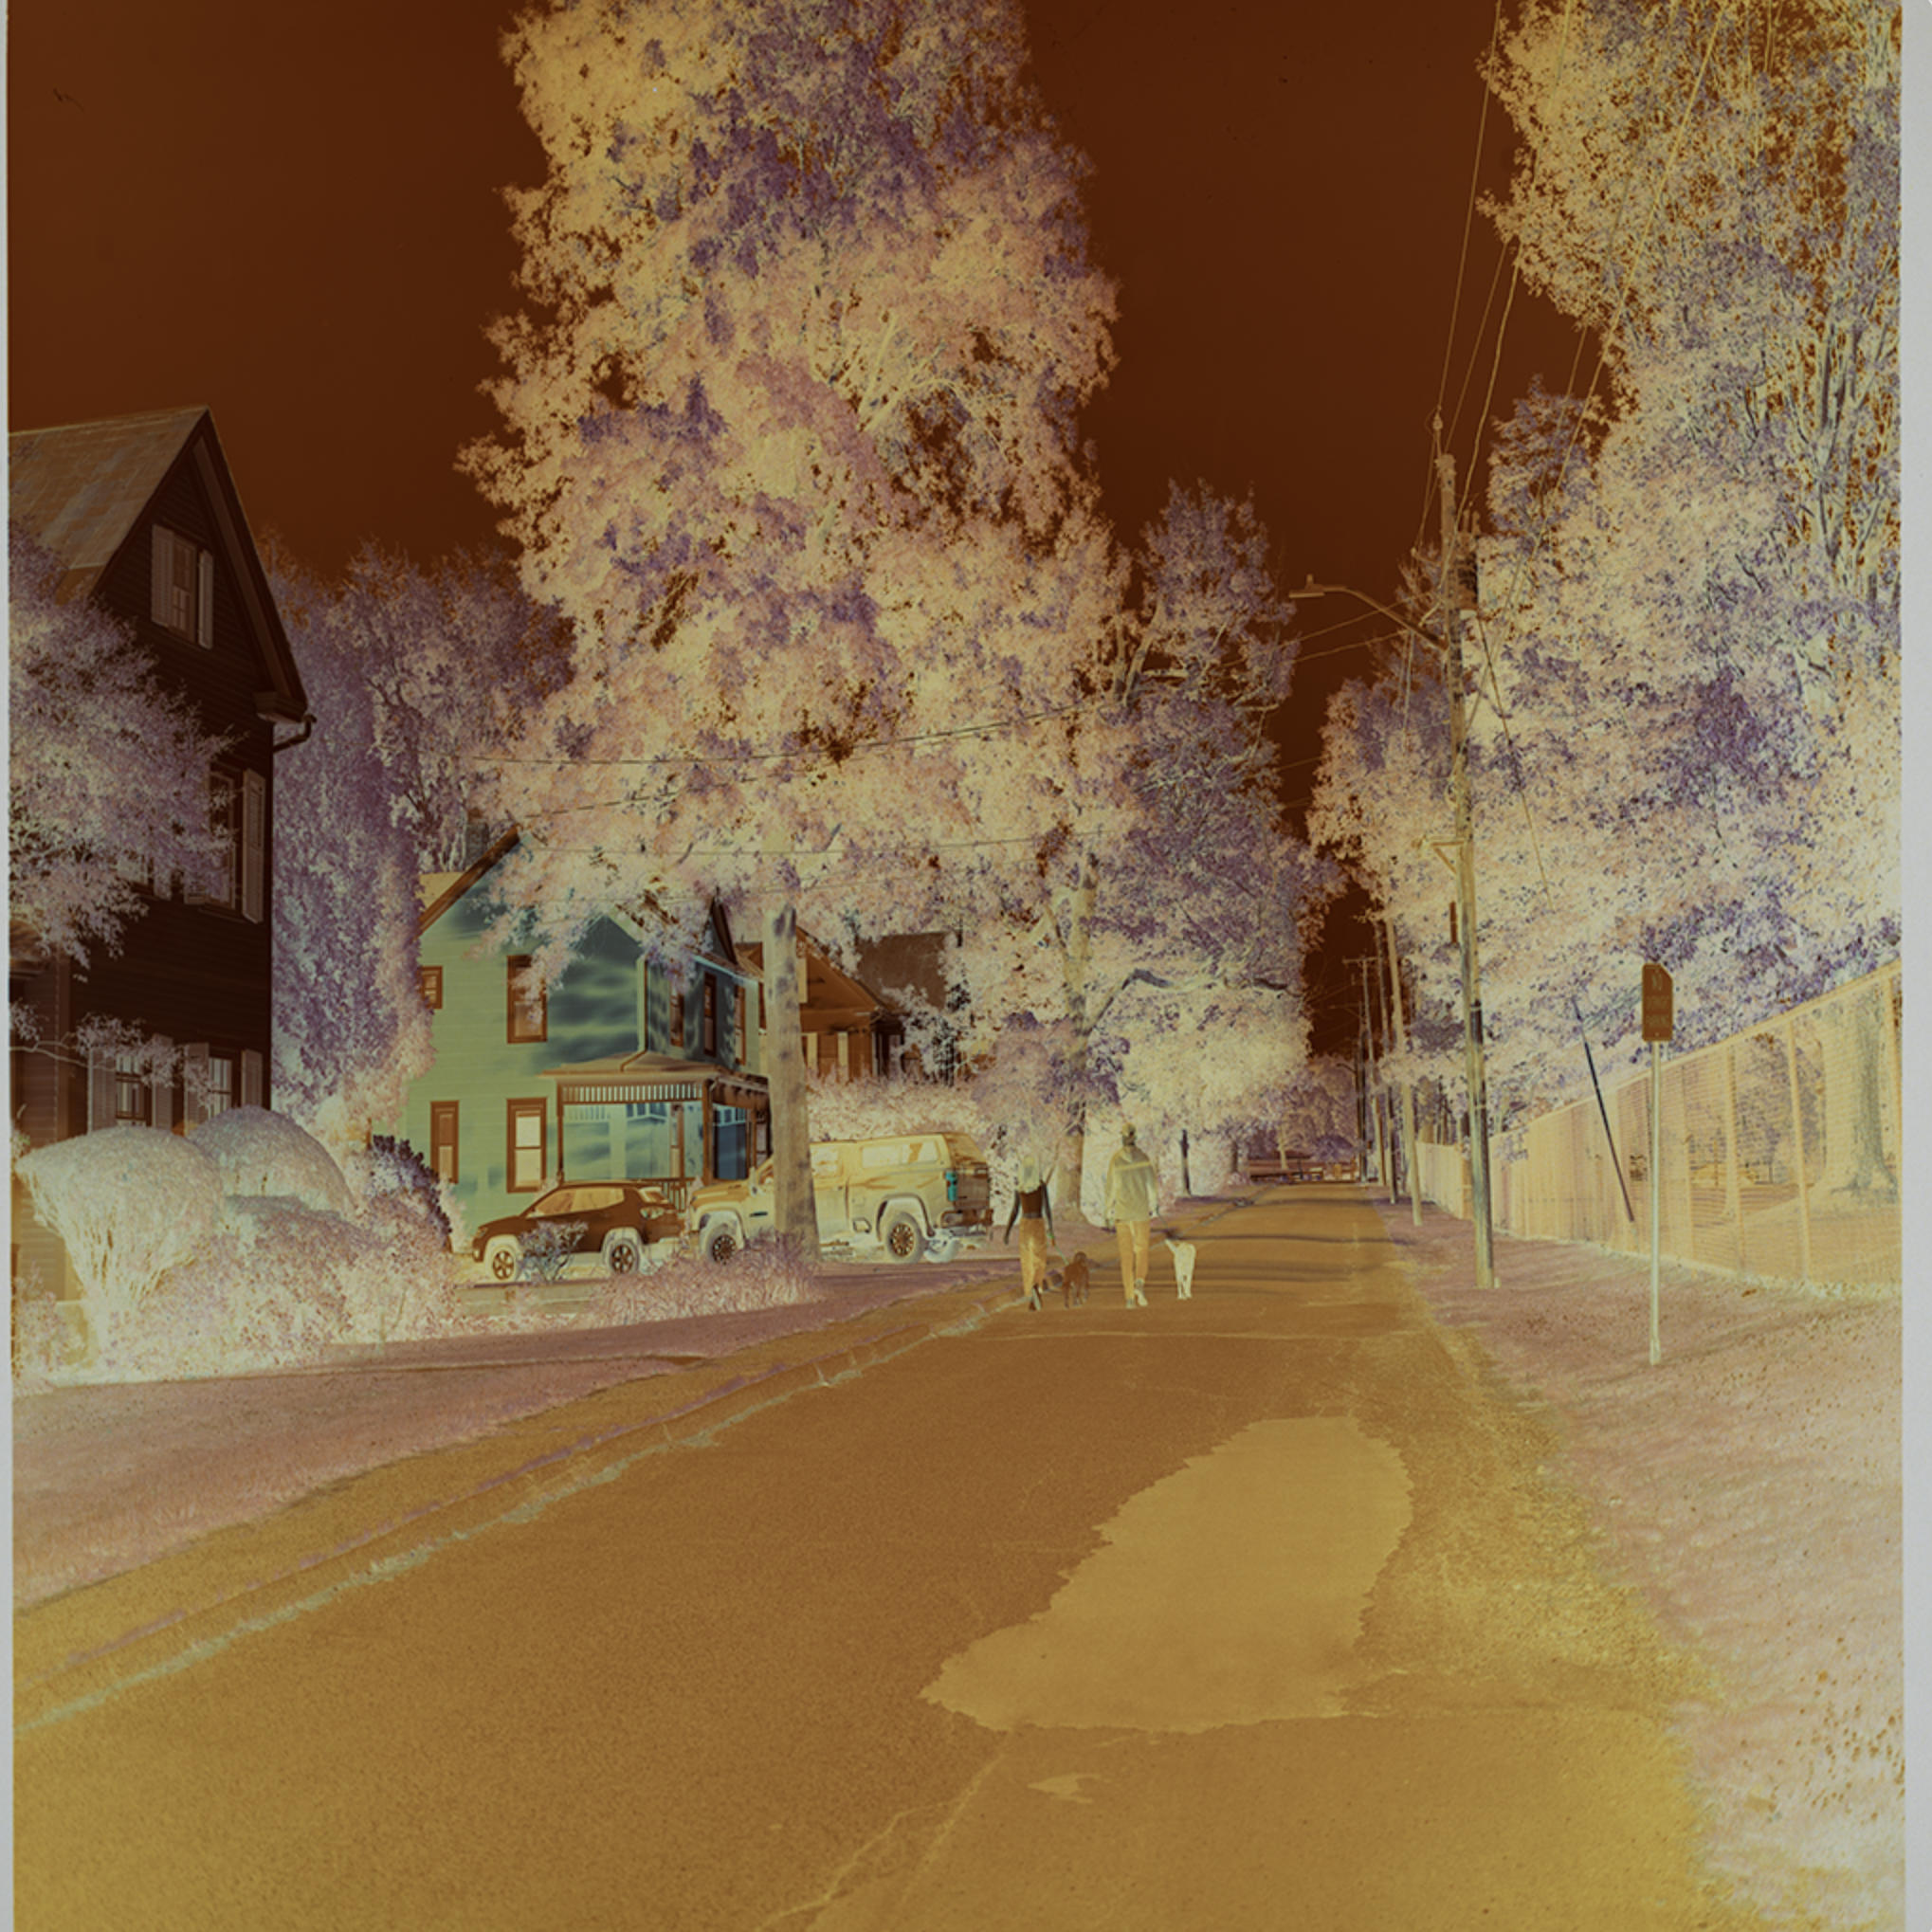
\includegraphics[width=0.4\linewidth]{testneg.png}
	\caption{A sample test image}
	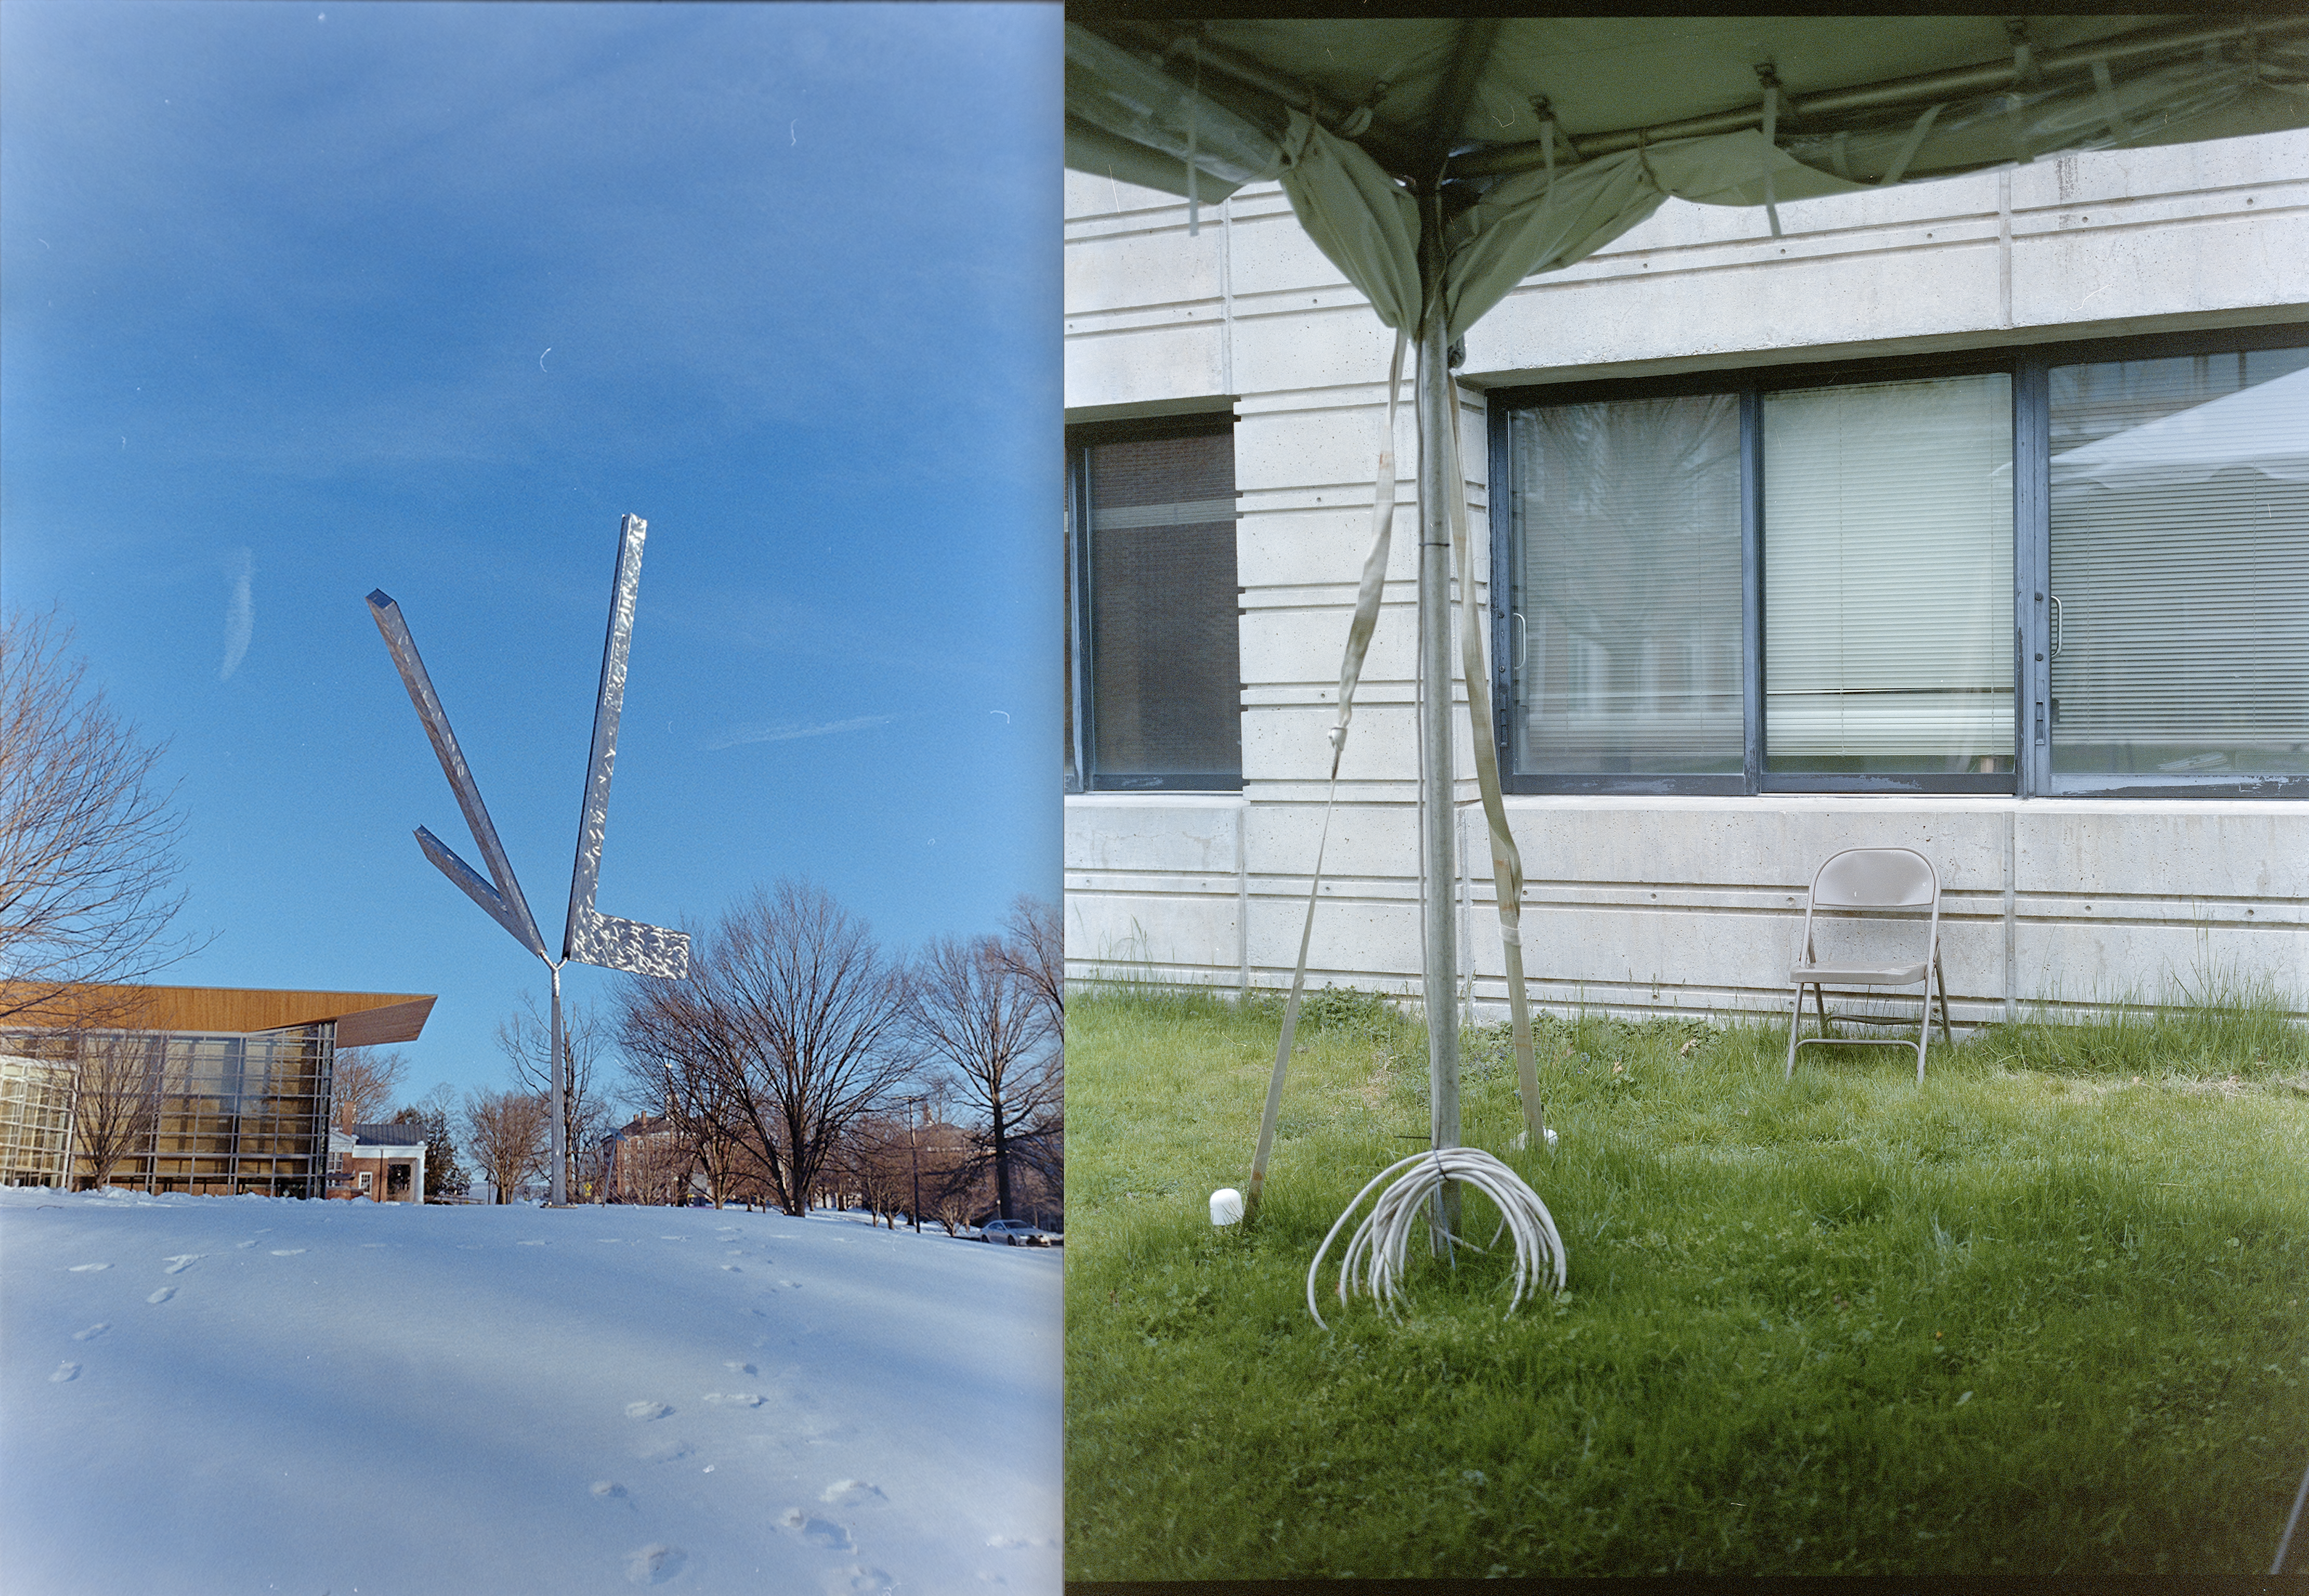
\includegraphics[width=0.6\linewidth]{dist.png}
	\caption{Ditribution shift between overcast fall afternoon, and bright winter morning}
	\label{fig:test}
\end{figure}

\begin{figure}
	\centering
	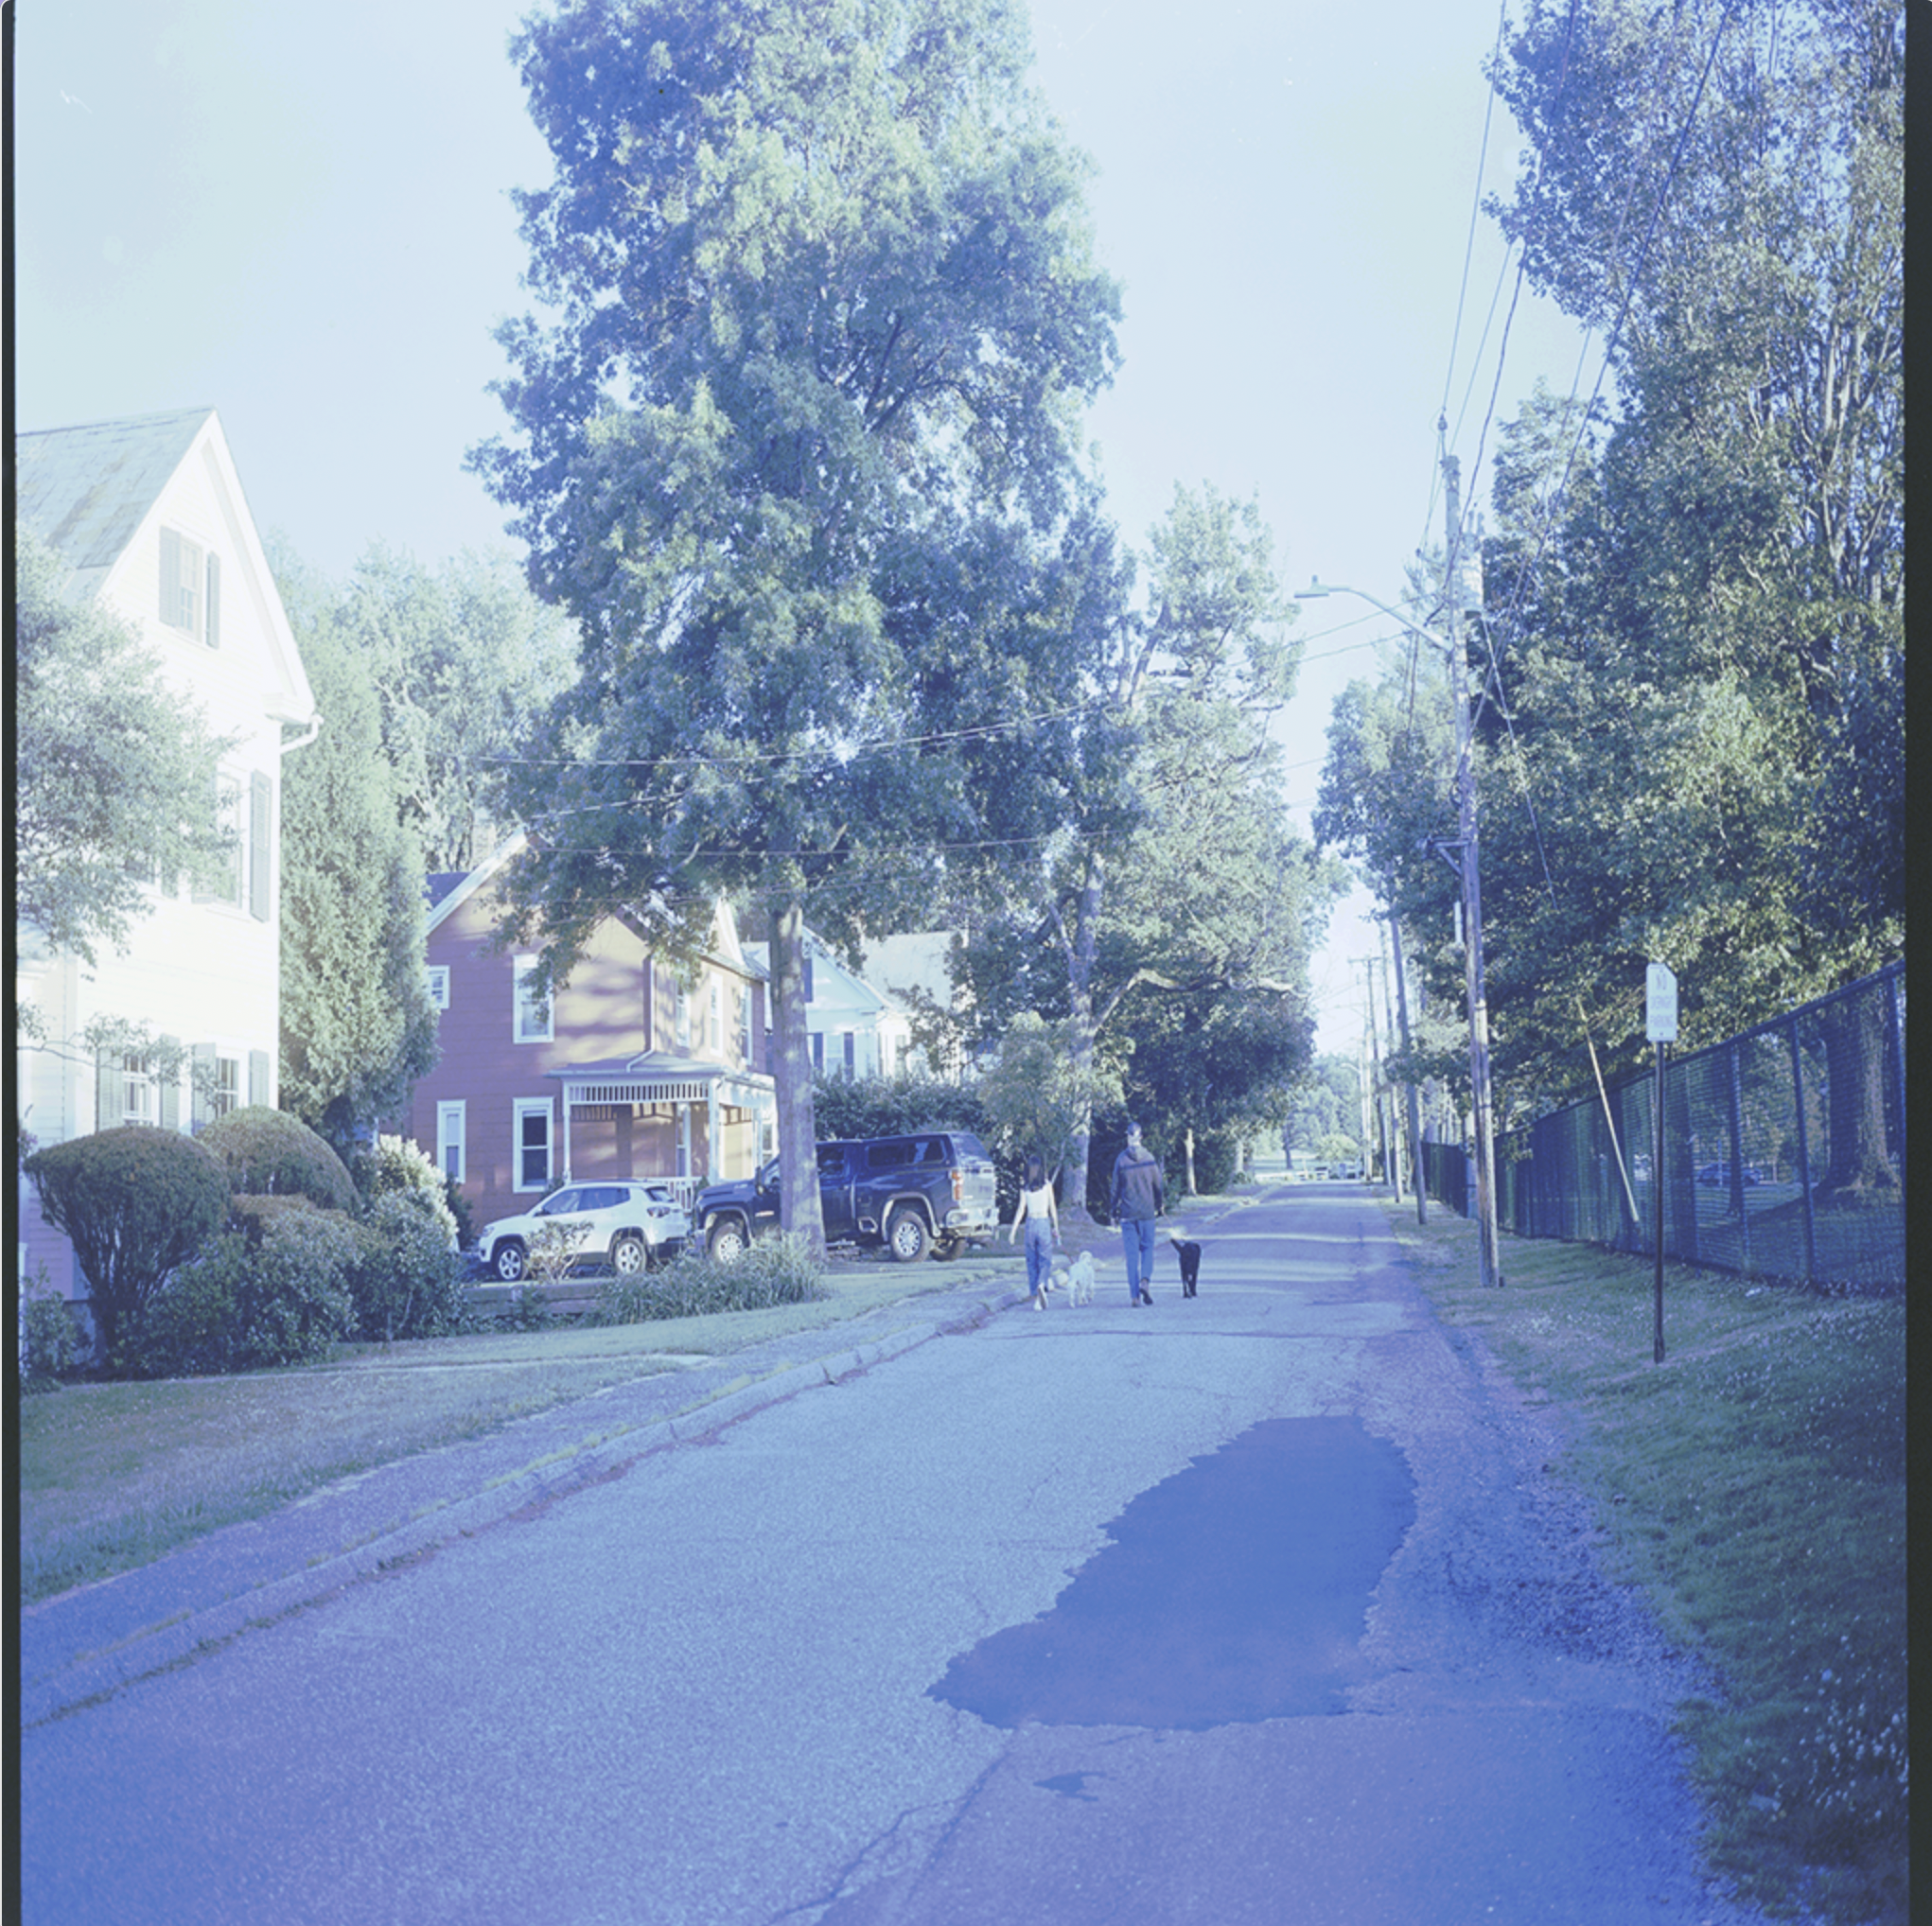
\includegraphics[width=0.4\linewidth]{gbres.png}
	\caption{Result generated by the GB model}
	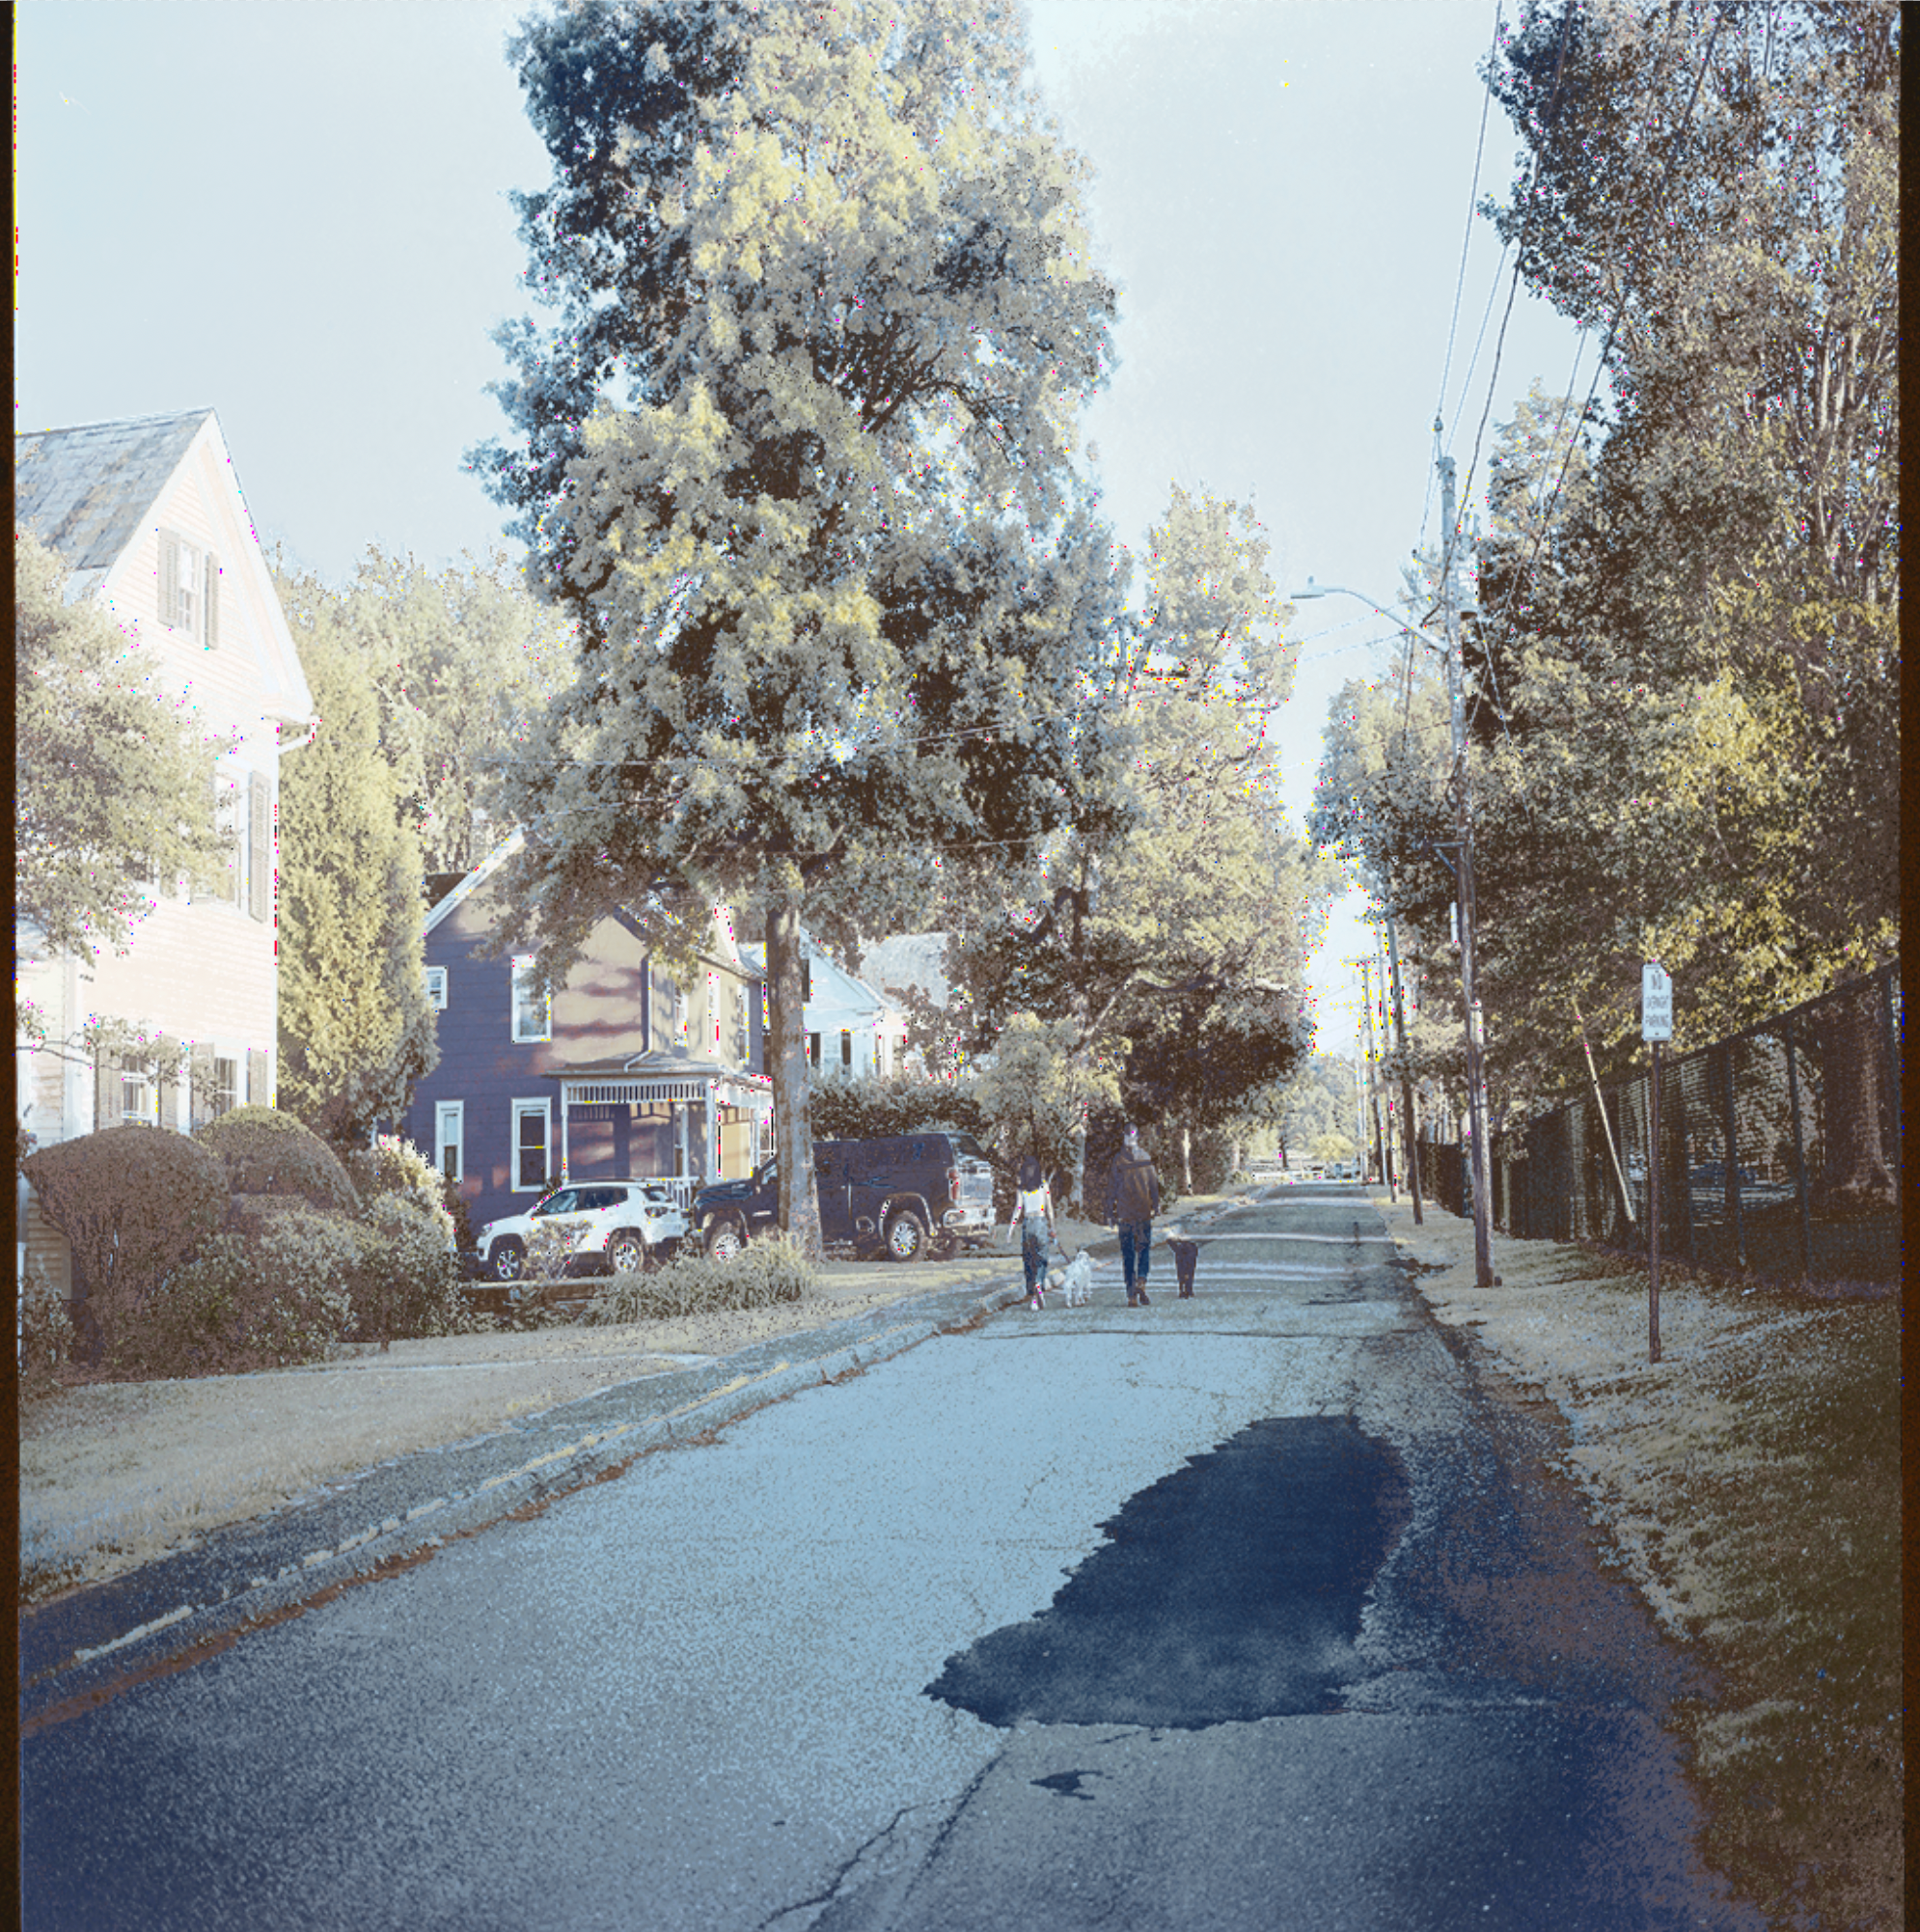
\includegraphics[width=0.4\linewidth]{dnnres.png}
	\caption{Result generated by the sparse autoencoder}
	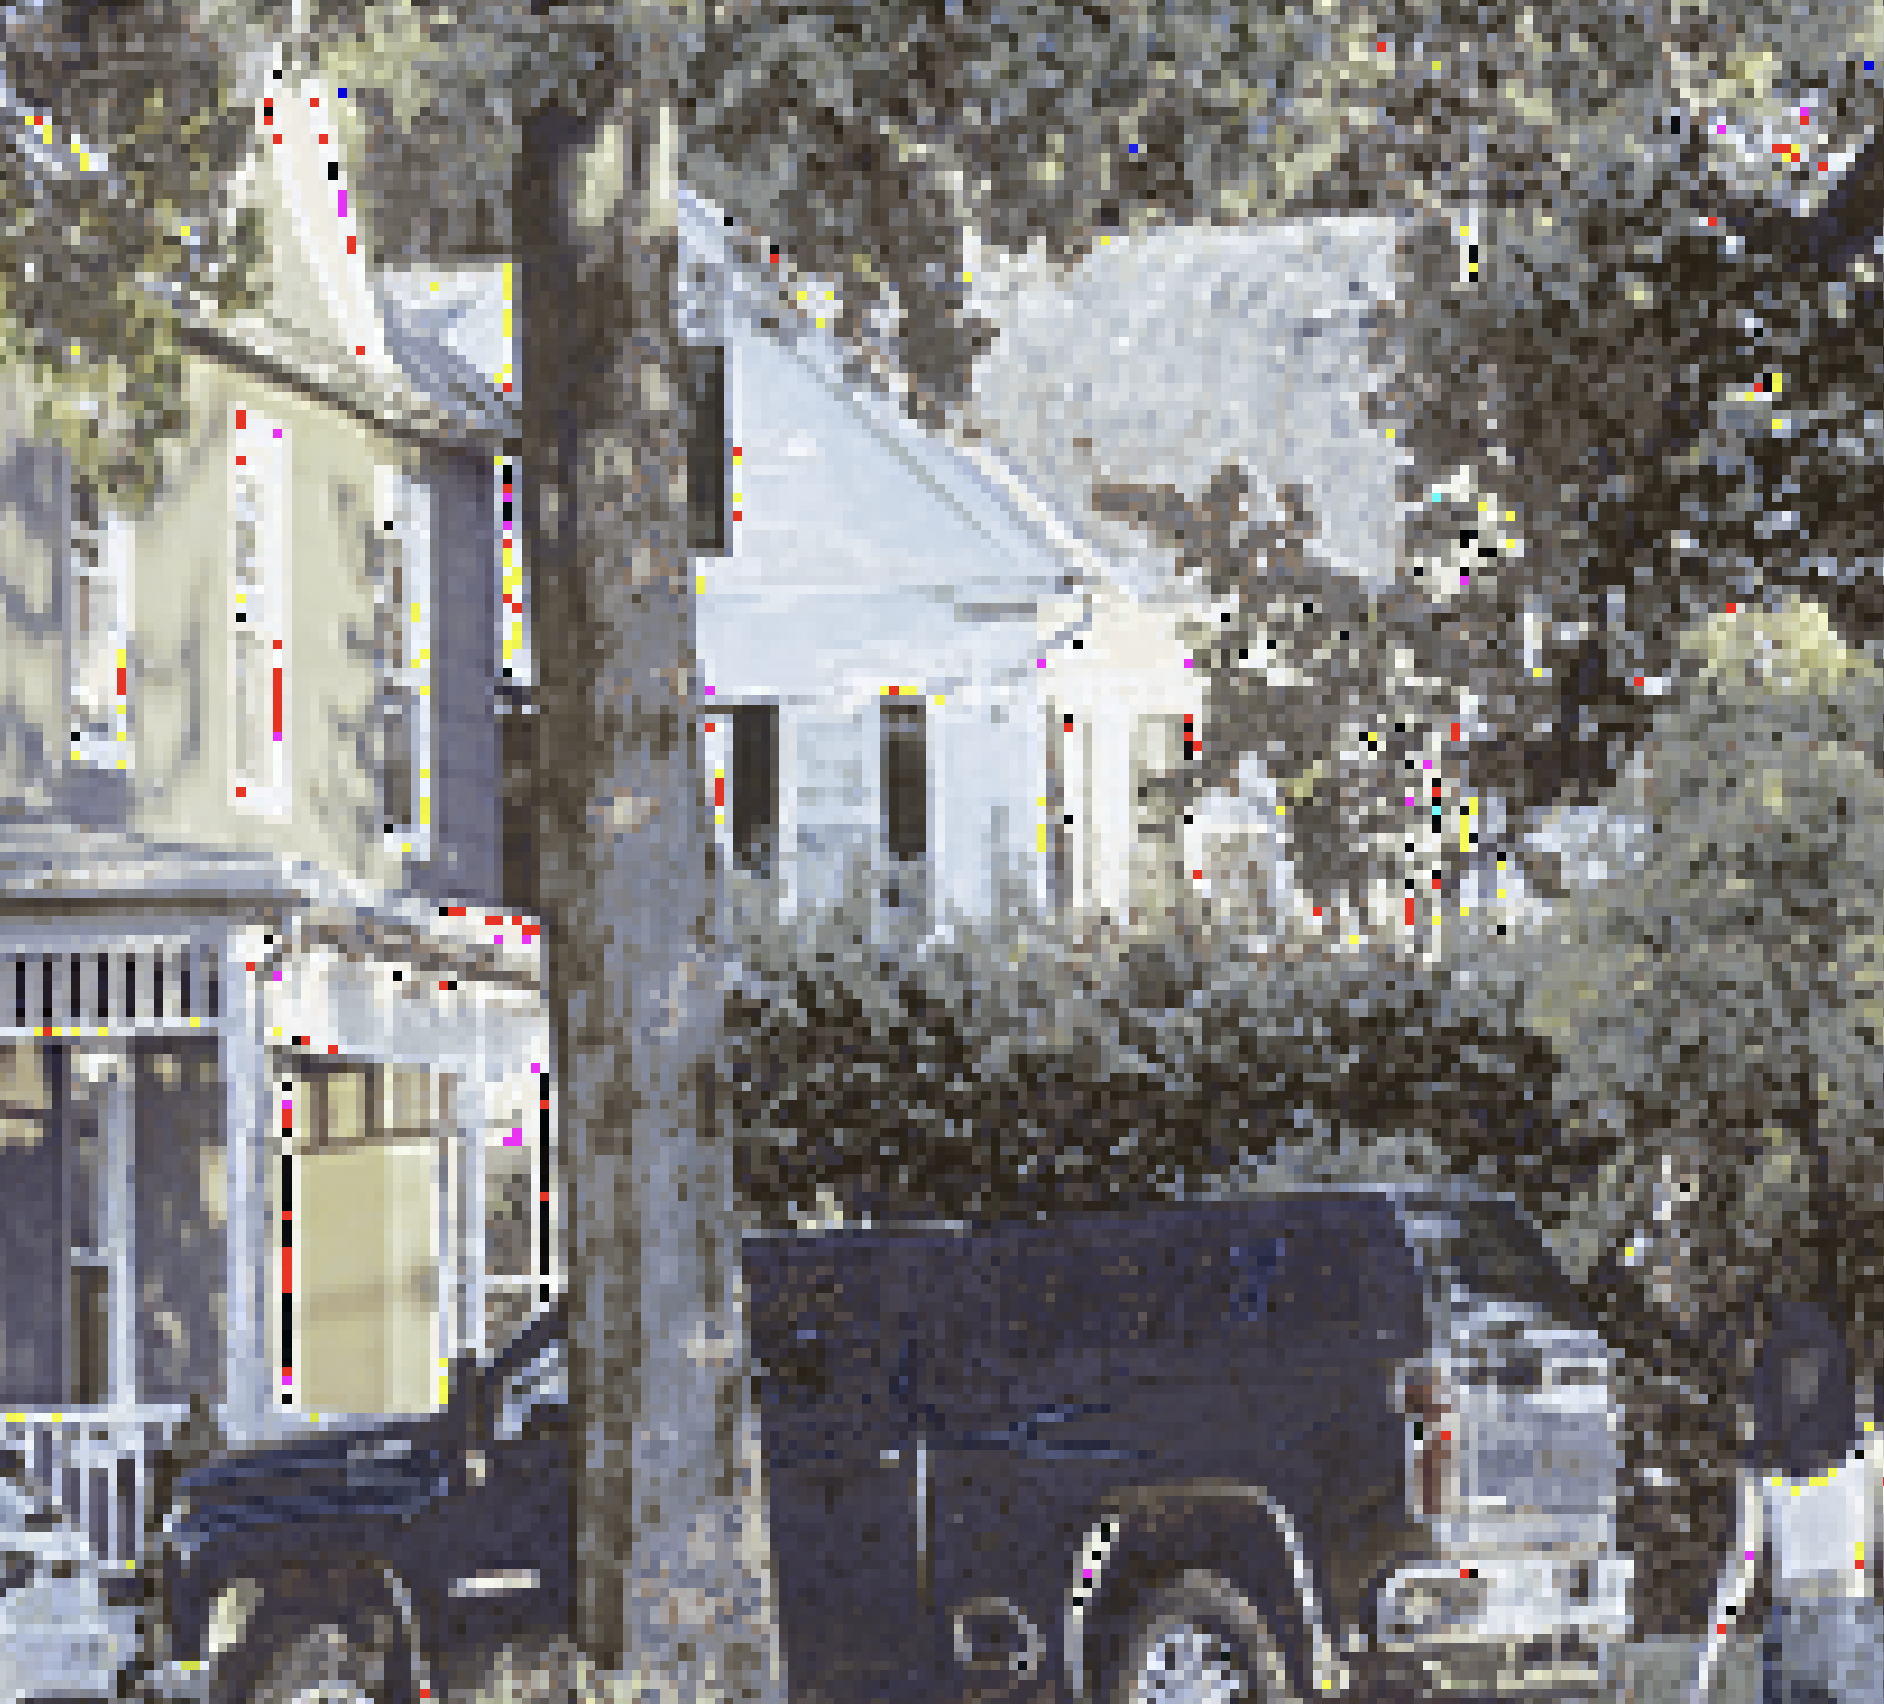
\includegraphics[width=0.4\linewidth]{artifact.png}
	\caption{Enlargement showing visual artifacts in the image above}
	\label{fig:res}
\end{figure}

\begin{figure}
	\centering
	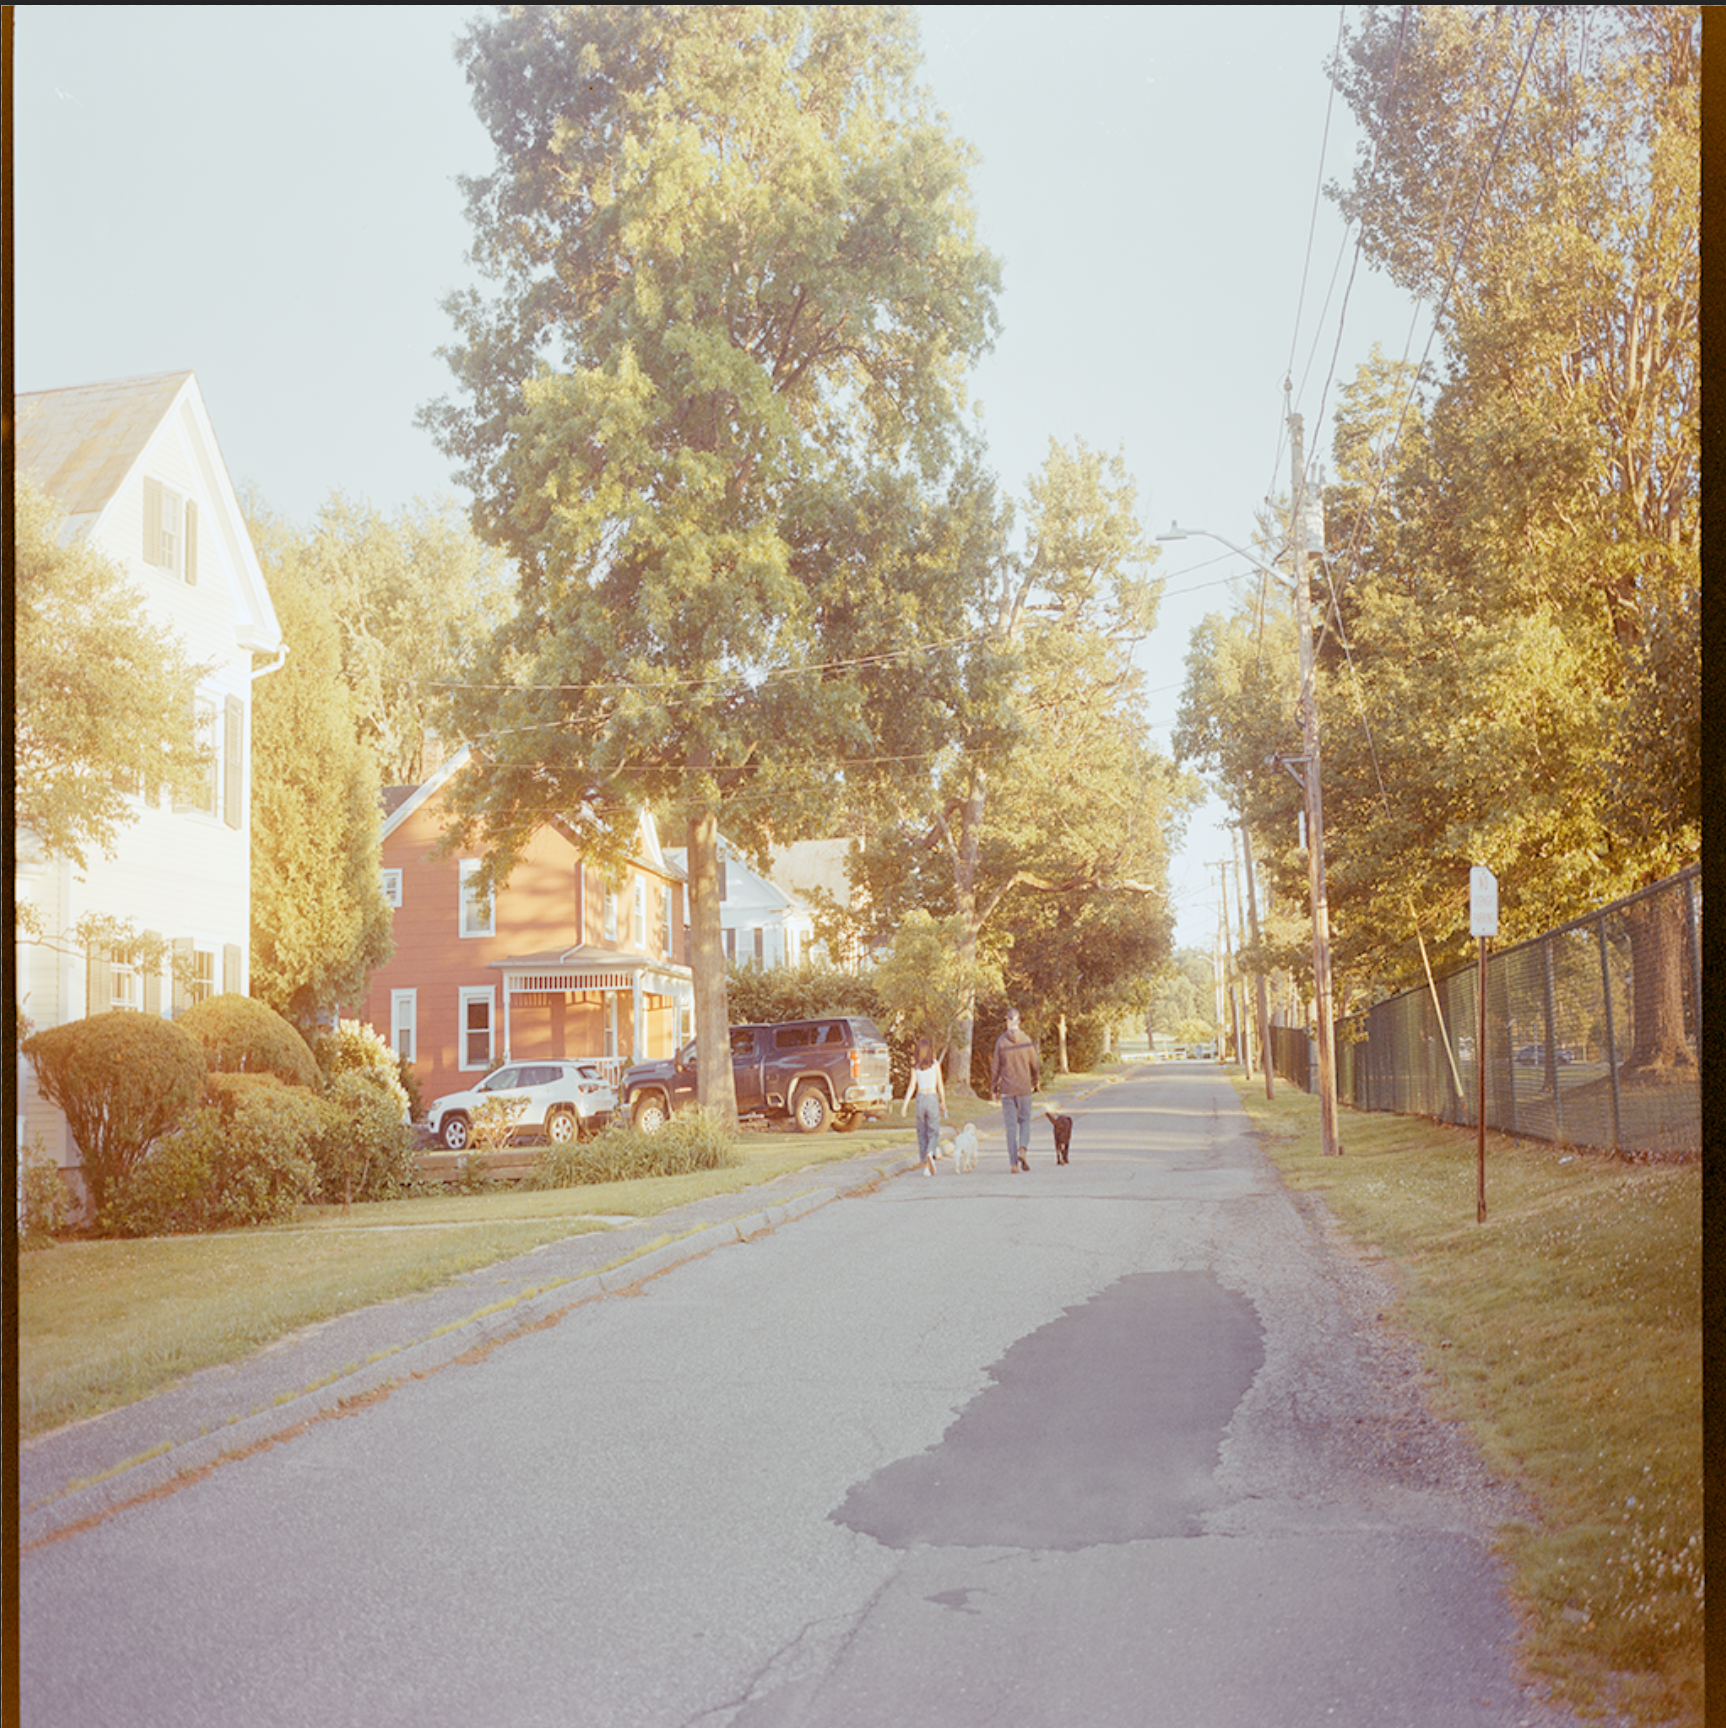
\includegraphics[width=0.4\linewidth]{manual.png}
	\caption{Manual inversion of the same negative}
	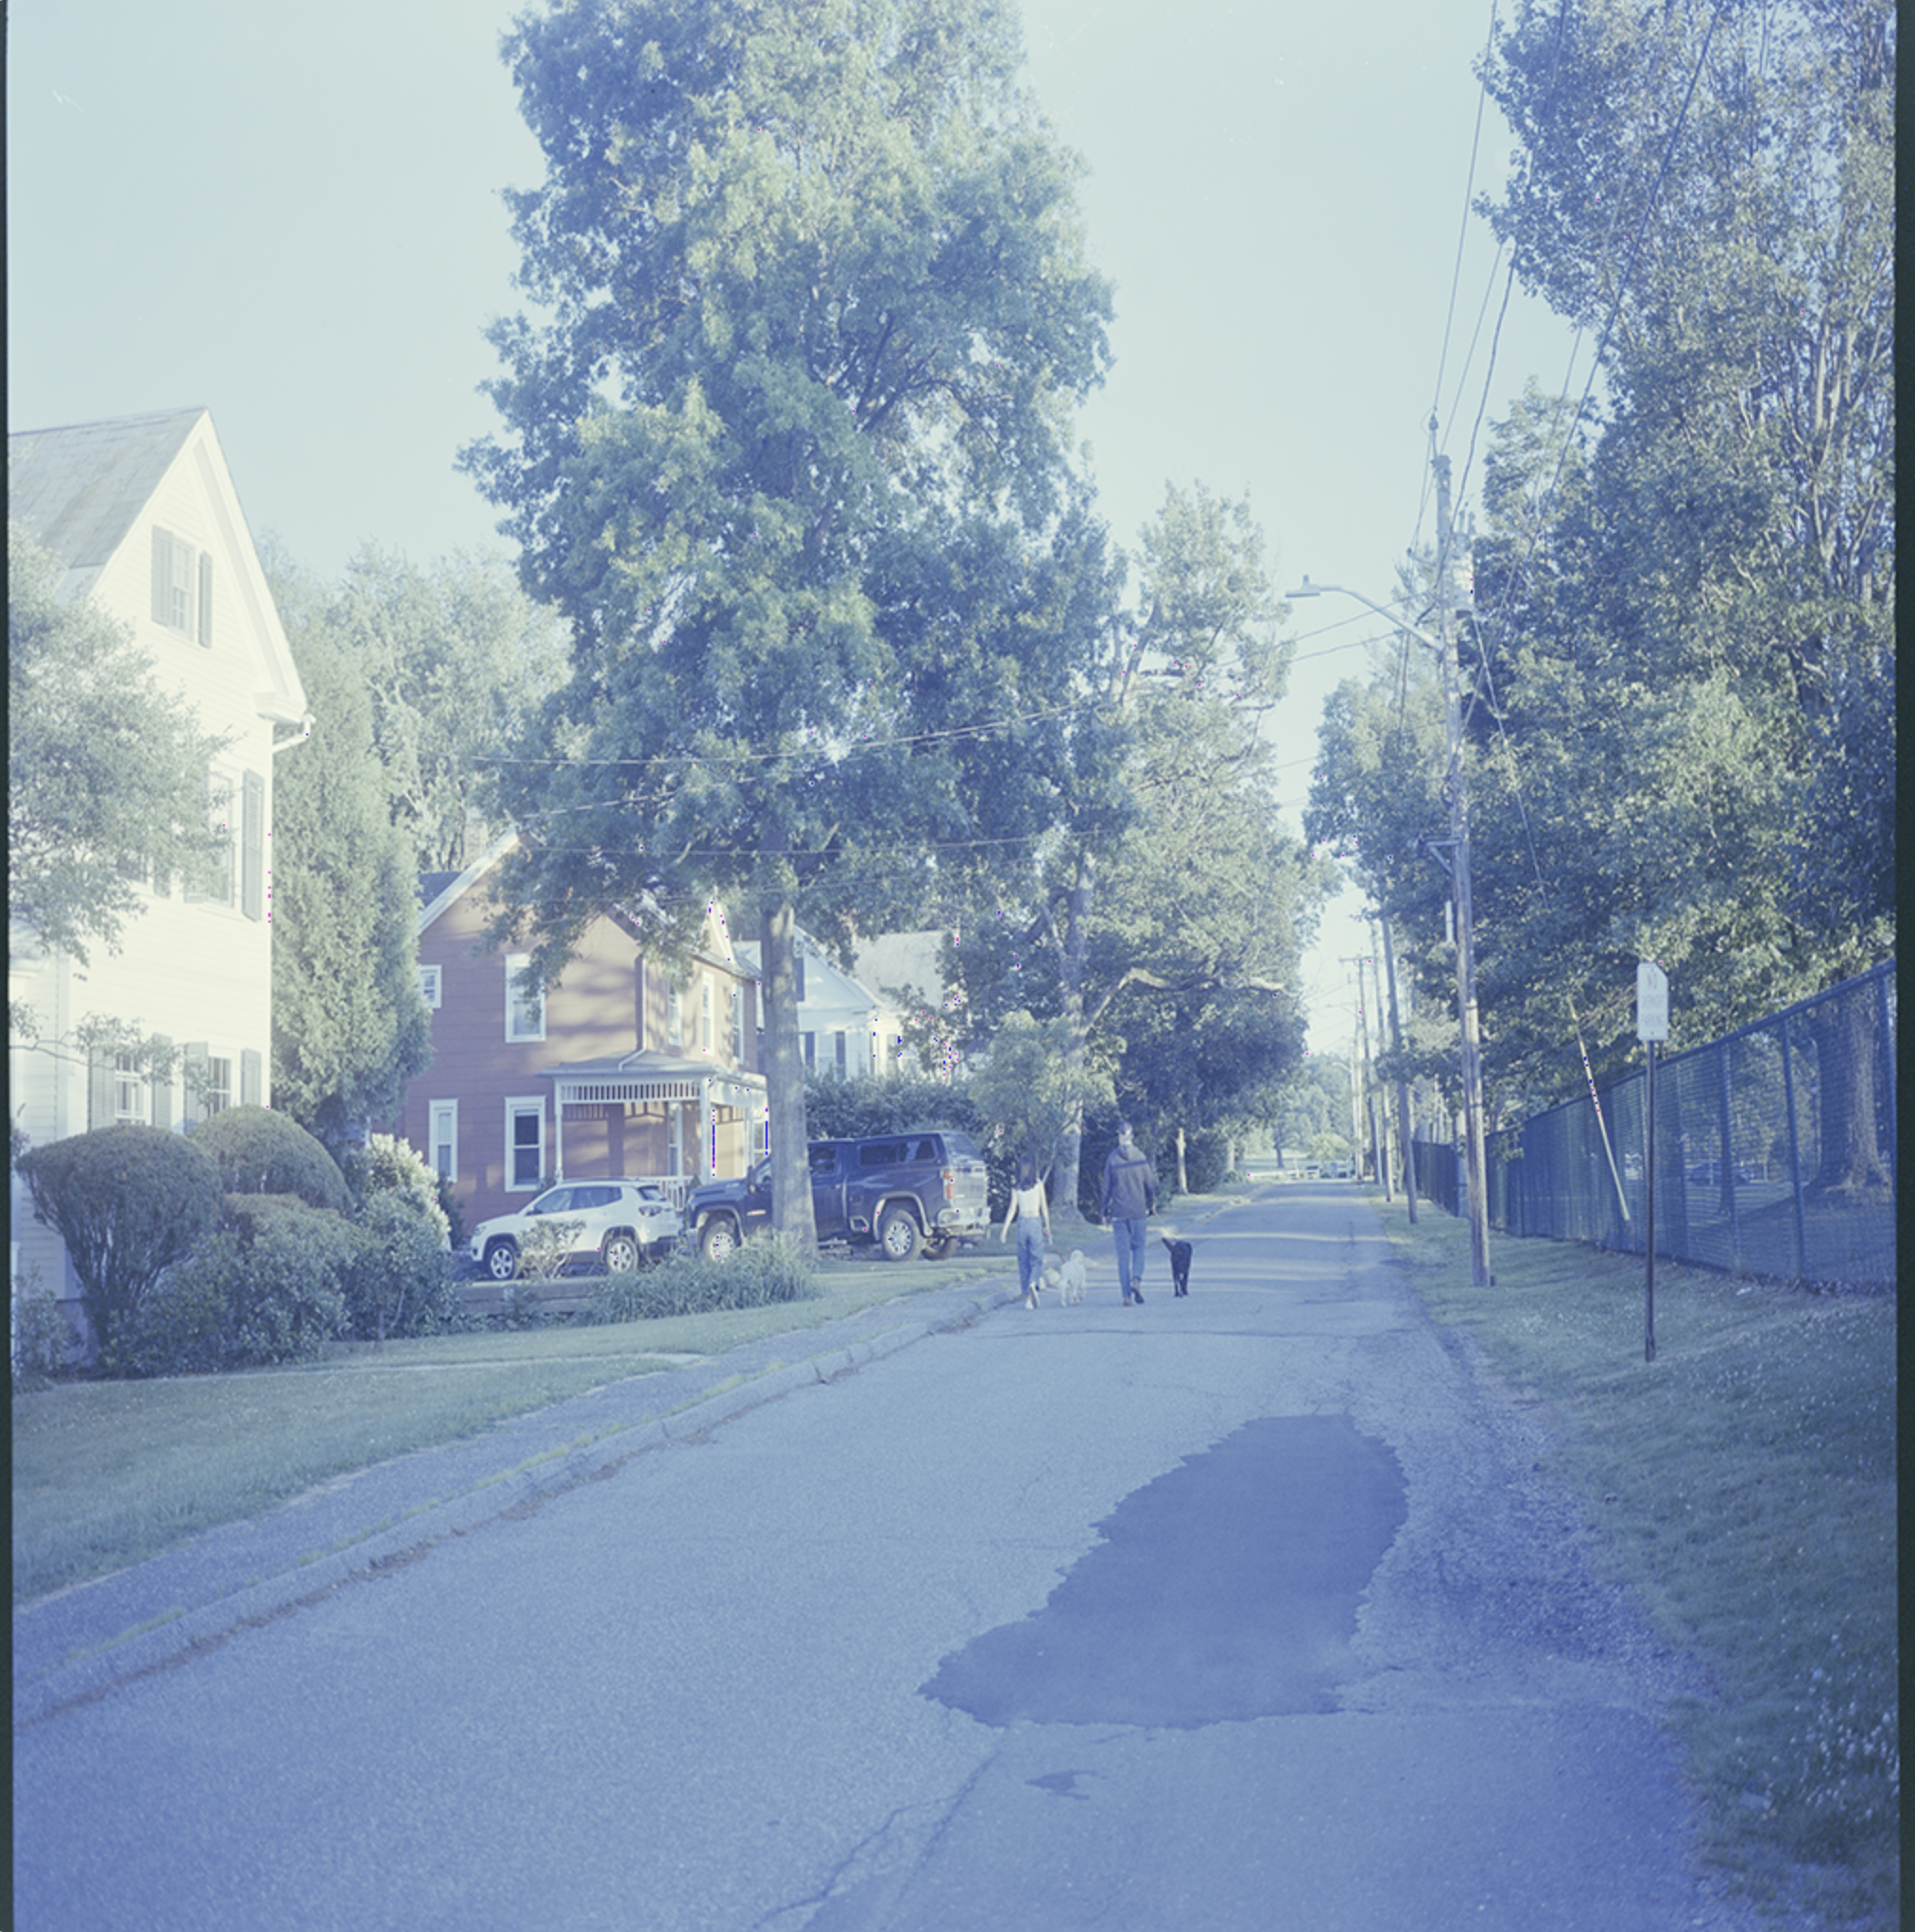
\includegraphics[width=0.4\linewidth]{rgbdnn.png}
	\caption{Result from simple MLP model B}
\end{figure}
%%%%%%%%%%%%%%%%%%%%%%%%
% Results
%%%%%%%%%%%%%%%%%%%%%%%%
\section{Ablation Study}
\label{sec:ablation}
I performed the ablation study by reducing amount of data.

To reduce the amount of data, I scaled the dataset to 1/16th its original size, and retrained the model. 
The performance of this model is shown in the table below:

\begin{center}
	\begin{tabular}{ c|c|c|c }
	 &  \textbf{Train Accuracy}& \textbf{Validation Accuracy} & \textbf{Test Accuracy} \\
	 \hline
	 \textbf{Regular-size data} & 0.8847 & 0.7895 & 0.6821 \\  
	 \hline
	 \textbf{Reduced-size data} & 0.8182 & 0.7187 & 0.6093 \\

	\end{tabular}
	\end{center}

	As we can see the performance of the model is lower when trained with a smaller dataset. 
	This is fair because the model is attempting to learn the mapping between pixel values, and for 
	16-bit images in the dataset, there would be $2^{48}$ total colors to be learned 
	(which could also be a good thing, since it would be very difficult to build an overparameterized network for this task). 
	Therefore, limiting 
	the size of the training set should limit the model's ability to learn accurately. However, we do observe that the 
	performance of the model is not severelly degraded, which could imply that our model is indeed learning to generalize 
	an underlying function, and not just memorizing the mapping between pixel values it has seen.

%%%%%%%%%%%%%%%%%%%%%%%%%
% Discussion + Conclusion
%%%%%%%%%%%%%%%%%%%%%%%%%
\section{Discussion and Conclusion}
\label{sec:discussion}
Although accuracy metrics are promising, I do not think that the current model is suitable for deployment in this application which requires critial color accuracy.
Beyond the issue of visual artifacts, one other potential issue I have noticed in this project is the problem of white balance. 
Specifically, the color white is presented as different colors under different lighting conditions. 
In the darkroom, correcting white balance requires trial-and-errors, often passing the image through color-correcting filters. 
However, since all inverted images in my dataset have been corrected for white balance, this could introduce a 
subtle distribution shift that confuses the model. To move toward a more accurate and realistic model in the future, I might attempt to, 
counterintuitively, build a model that less resembles the color-corrected image but more honestly reflect the state of the film negative before color correction.
%%%%%%%%%%%%%%%%%%%%%%%%%
% References
%%%%%%%%%%%%%%%%%%%%%%%%%
\newpage
\bibliography{references}


\end{document}

